\documentclass[a4paper,11pt]{scrartcl}
\usepackage[T1]{fontenc}
\usepackage[utf8]{inputenc}
\usepackage{lmodern}
\usepackage[spanish]{babel}
\usepackage{mathtools}
\usepackage{amssymb, amsmath, amsbsy}
\usepackage{float}
\usepackage{enumerate}
\usepackage{graphicx}
\usepackage{subfigure}
\usepackage{hyperref}

\title{Cinética de la partícula}
\subtitle{Segundo Examen Parcial \\ Equipo 12}
\author{
  Aguilar Enriquez Paul Sebastian\\
  \and
  Benitez Barroso Brandon Raul\\
  \and
  Castillo Herrera Gabriela\\
  \and
  Martinez Vidal Joceline Yadira\\
  \and
  Milán Hernández Maria Fernanda
  }
\date{26 de septiembre del 2016}
\begin{document}

\maketitle

\begin{center}
  Repositorio del documento en GitHub
  \url{https://github.com/penserbjorne/clase-cinematicaydinamica-2017-1}
\end{center}

\textbf{Ejercicio 14} El resorte que conecta el soporte A y el collarín de masa ${\bf m}$  en B de la figura~\ref{fig:14_1}, tiene constante  ${\bf k}$. Suponiendo que la longitud sin elongación del resorte es  ${\bf l}$, calcula la velocidad de la masa en el punto C si el collarón se suelta el reposo en $x = x_{0} $.\\

\begin{figure}[H]
  \centering
  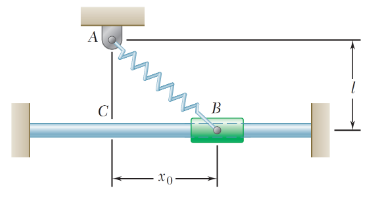
\includegraphics[height=4cm]{14_1}
  \caption{Sistema mostrado para el Problema 14.}
  \label{fig:14_1}
\end{figure}

\textbf{Solución:}

\begin{center}

Poniendo el origen en el punto C y sea x positvo a la derecha. Después ponemos a x en una posición coordinada del deslizador B y $x_{0}$ en su valor inicial. \\

\begin{figure}[H]
  \centering
  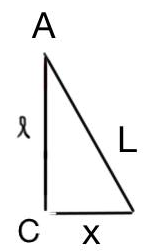
\includegraphics[height=4cm]{14_2}
  \caption{Geometria con respecto al punto C.}
  \label{fig:14_2}
\end{figure}

\begin{center}
$L =  \sqrt{l^{2} + x^{2}}  $ \\
\end{center}
La enlogación del resorte es $ e = L -1 $ y la magnitud de la fuerza ejercida por el resorte es: \\
\begin{center}
$F_{s} = ke = k( \sqrt{l^{2} + x^{2}} - l )  $ \\
\end{center}
Por geometría:\\
\begin{center}
$\cos (\theta) = \dfrac{x}{\sqrt{l^{2} + x^{2}}}  $ \\
\[
\sum F_{x} = ma_{x} = -  F_{x} \cos (\theta)  = ma
\]
\\
$ -  k( \sqrt{l^{2} + x^{2}} - l ) (\dfrac{x}{\sqrt{l^{2} + x^{2}}}) = ma $\\ 
 $ a = - \dfrac{k}{m}(x - \dfrac{lx}{\sqrt{l^{2} + x^{2}}}) $\\
$ \int_{0}^{v} v dv = \int_{x_0}^{0} a dx $\\
$\dfrac{1}{2}v^{2} |_0^v =  - \dfrac{k}{m}  \int_{x_0}^{0} (x - \dfrac{lx}{\sqrt{l^{2} + x^{2}}}) dx =  - \dfrac{k}{m}(\dfrac{1}{2}x^{2} - l  \sqrt{l^{2} + x^{2}} ) |_{x_{0}}^v $\\
$ \dfrac{1}{2}v^{2} =   - \dfrac{k}{m}(0 -  l^{2} - \dfrac{1}{2}{x_{0}}^{2} + l  \sqrt{l^{2} +{x_{0}}^{2}} )  $\\
$ v^{2} = \dfrac{k}{m}(2 l^{2} + {x_{0}}^{2} - 2l  \sqrt{l^{2} +{x_{0}}^{2}} )  $\\
$ v^{2} = \dfrac{k}{m}(( l^{2} + {x_{0}}^{2})  - 2l  \sqrt{l^{2} +{x_{0}}^{2}} + l^{2}) $\\
\end{center}
Por lo tanto, la velocidad es: \\
\begin{equation}
  \left\lbrace
  \begin{array}{l}
    v = \sqrt{\dfrac{k}{m}}( \sqrt{l^{2} +{x_{0}}^{2}} - l )
  \end{array}
  \right.
\end{equation}

\end{center}

\textbf{Ejercicio 20} Los bloques mostrados en la figura~\ref{fig:20_1} son liberados desde el reposo. Suponiedo que el coeficiente de friccón entre el bloque A y el piso es cero (i.e. no hay fricción), que la polea no tiene masa y que la cuerda que los une es intextensible, encuentra la aceleración de cada bloque. \\

\begin{figure}[H]
  \centering
  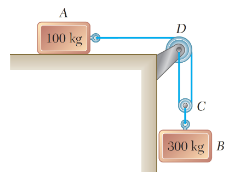
\includegraphics[height=4cm]{20_1}
  \caption{Sistema mostrado para el Problema 20.}
  \label{fig:20_1}
\end{figure}

\textbf{Solución:}

\begin{center}

En el caso de que si el bloque A si desliza hacia la derecha, el bloque B desciende.\\
d = distancia.\\

\begin{figure}[H]
  \centering
  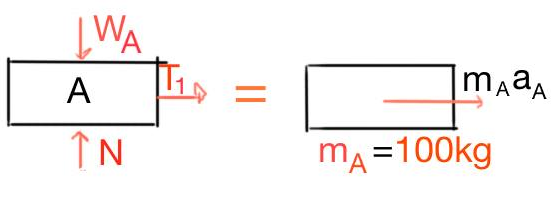
\includegraphics[height=3cm]{20_2}
  \caption{Diagrama de cuerpo libre de A.}
  \label{fig:20_2}
\end{figure}

\begin{figure}[H]
  \centering
  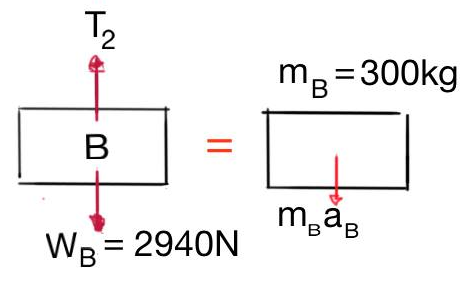
\includegraphics[height=4cm]{20_3}
  \caption{Diagrama de cuerpo libre de B.}
  \label{fig:20_3}
\end{figure}

\begin{center}
$d_{B} =  \dfrac{1}{2} d_{A} $ \\
\end{center}
Por lo que al tener la distancia, al derivarla dos veces tenemos que la aceleración es:
\begin{center}
\begin{equation}
a_{B} = \dfrac{1}{2} a_{B}
\end{equation}
\end{center} 
Para la tensión de la cuerda ACD, tenemos que es:\\
\begin{center}
\[
\sum F_{x} = ma_{A}a_{A}
\]
\begin{equation}
 T_{1} = 100a_{A}
\end{equation}
\end{center} 
Tenemos que el peso del bloque B es:\\
\begin{center}
$W_{B} = m_{B}g = (300 kg)(9.81 m/s^{2}) = 2940 N $ \\
\end{center}
Para la tensión de la vuerda BC, tenemos que:\\
\begin{center}
\[
\sum F_{y} = ma_{B}a_{B}
\]
 $ 2940 - T_{2} = 300a_{B} $
\end{center} 
Y al suistituir $ a_{B} $ de (1), tenemos que:\\
\begin{center}
$ 2940 -  T_{2} = 300(\dfrac{1}{2}a_{A}) $\\
\begin{equation}
 T_{2} = 2940 - 150a_{A}
\end{equation}
\end{center} 
Ahora, para la polea C, suponiendo que su masa es cero, tenemos que:
\begin{center}
\[
\sum F_{y} = ma_{C}a_{C} = 0
\]
\begin{equation}
 T_{2} - 2T_{1}= 0
\end{equation}
\end{center}
Sustituimos $ T_{1} y T_{2} $ de (2) y de (3) respectivamente, en (4), tenemos que:  \\
\begin{center}
$ 2940 -  150a_{A} - 2(100a_{A}) = 0 $ \\
$ 2940 - 350a_{A} = 0 $ \\
Por lo que $ a_{A}= 8.40  \dfrac{m}{s^{2}}$\\
\end{center}
Y para la aceleración B, tenemos que:
\begin{center}
$ a_{B} = \dfrac{1}{2} a_{A} =  \dfrac{1}{2}(8.40 m/s^{2}) $\\
Por lo que $ a_{B}= 4.20  \dfrac{m}{s^{2}}$\\
\end{center}
Y por lo tanto la tensión 1 es:\\
\begin{center}
$  T_{1} = 100a_{A} = (100 kg)(8.40 m/s^{2}) $\\
Por lo que $  T_{1} = 840 N $
\end{center} 
De la (4), tenemos que para la tensión 2, es:\\
\begin{center}
$  T_{2} = 2T_{1} = (2)(840 N) $\\
Por lo que $  T_{2} = 1680 N $\\
\end{center}
Por lo tanto las aceleraciones del bloque A y B, son:\\
\begin{equation}
  \left\lbrace
  \begin{array}{l}
     a_{A}= 8.40  \dfrac{m}{s^{2}}\\
\\
    a_{B}= 4.20  \dfrac{m}{s^{2}}\\
  \end{array}
  \right.
\end{equation}

 
\end{center}

\textbf{Ejercicio 22} Los bloques \textbf{A} y \textbf{B} mostrados en la figura~\ref{fig:22_1} tienen masas $m_A$ y $m_B$, respectivamente. Si el coeficiente de fricción cinético entre todas las superficies es $\mu_k$, determine la aceleración del bloque B cuando se ejerce una fuerza $\hat{P}$ como se observa en la figura. Evalúa tus resultados
cuando $m_A = 40 kg$, $m_B = 8 kg$, $\theta = 25$, $\mu_k = 0.15$ y $|\hat{P}| = 40 N$.\\

\begin{figure}[H]
  \centering
  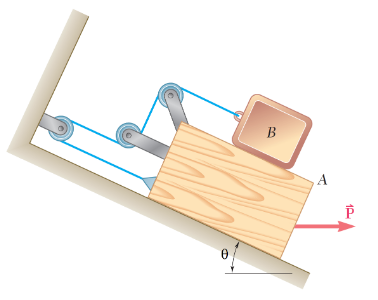
\includegraphics[height=4cm]{22_1}
  \caption{Sistema mostrado para el Problema 22.}
  \label{fig:22_1}
\end{figure}

\textbf{Solución:}

\begin{center}

Solucion

\end{center}

\textbf{Ejercicio 27} Miley Cyrus se volvió a subir a la bola de demolición que se muestra en la figura~\ref{fig:27_1}. Calcula la tensión de la cuerda cuando (a) la bola alcanza la máxima altura (en el punto \textbf{C}) y (b) la bola pasa por el punto \textbf{D} con una rapidez $ v = 4.2 \frac{m}{s}$. Supón que el cable entre los puntos \textbf{AB} mide 15
m y que la bola (junto con Miley) tiene una masa de 110 kg. \\

\begin{figure}[H]
  \centering
  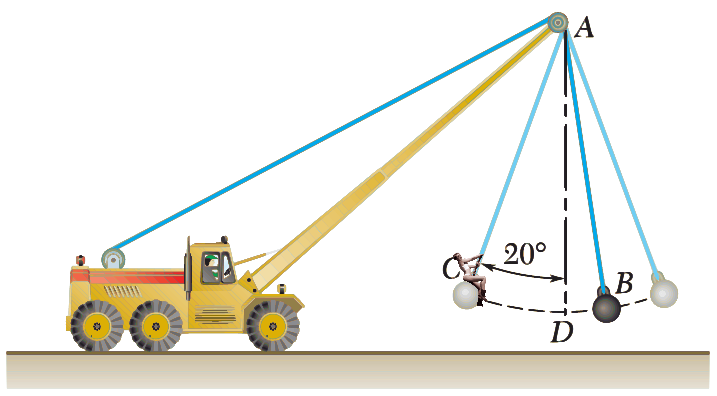
\includegraphics[height=4cm]{27_1}
  \caption{Sistema mostrado para el Problema 27.}
  \label{fig:27_1}
\end{figure}

\textbf{Solución:}

\begin{figure}[H]
  \centering
  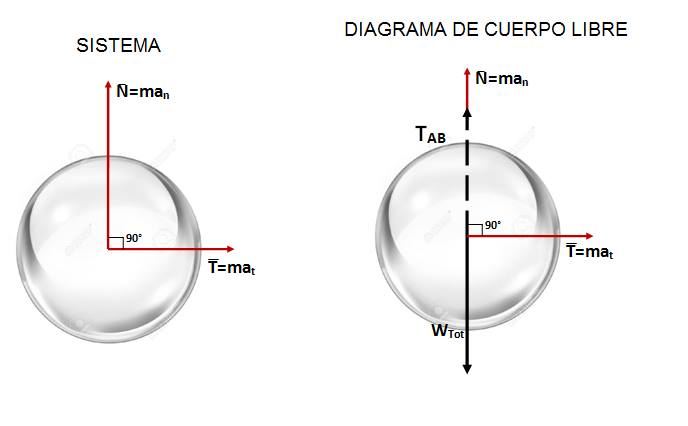
\includegraphics[height=6cm]{27_2}
%  \caption{}
  \label{fig:27_2}
\end{figure}

\begin{figure}[H]
  \centering
  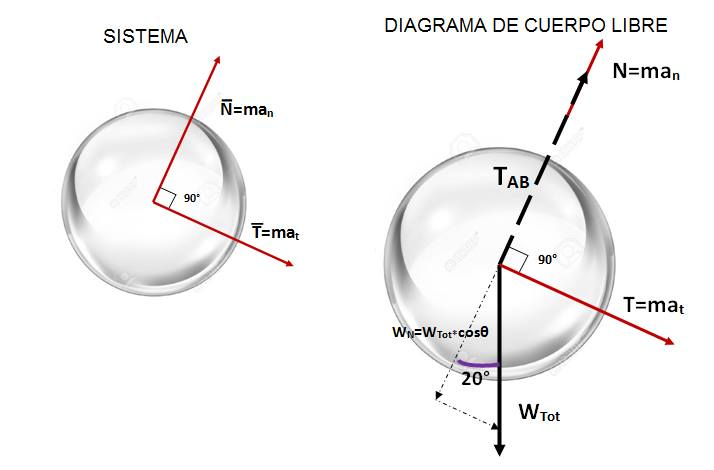
\includegraphics[height=6cm]{27_3}
%  \caption{}
  \label{fig:27_3}
\end{figure}

\begin{center}
a) $T_{BA}$ (Tension) en el punto C.\\
\hfill \break
$v_C = 0$\\
\hfill \break
$a_n = \frac{v_C^2}{L_{AB}} = 0$\\
\hfill \break
$\Sigma F_n = m_{tot} a_n = 0$\\
\hfill \break
$W_{tot} = m_{tot} g$\\
\hfill \break
$\Sigma F_n = T_{BA} - cos(\theta)w_{tot} = 0$\\
\hfill \break
$T_{BA} = cos(\theta)w_{tot}$\\
\hfill \break
$T_{BA} = [cos(20)][100 kg][9.81 \frac{m}{s^2}]$\\

\begin{equation}
  \left\lbrace
  \begin{array}{l}
    T_{BA} = 1014.0223 \frac{kg*m}{s} = 1014.0223 N
  \end{array}
  \right.
\end{equation}

b) $T_{BA}$ (Tension) en el punto D.\\
\hfill \break
$v_o = 4.2 \frac{m}{s}$\\
\hfill \break
$a_n = \frac{v_o^2}{L_{AB}}$\\
\hfill \break
$\Sigma F_n = m_{tot} a_n = m_{tot} \frac{v_o^2}{L_{AB}}$\\
\hfill \break
$\Sigma F_n = T_{BA} - w_{tot} = m_{tot} a_n$\\
\hfill \break
$T_{BA} - w_{tot} = m_{tot} \frac{v_o^2}{L_{AB}}$\\
\hfill \break
$T_{BA} = m_{tot} \frac{v_o^2}{L_{AB}} + w_{tot}$\\
\hfill \break
$T_{BA} = [110 kg] \frac{(4.2 \frac{m}{s})^2}{15 m} + [110 kg][9.81 \frac{m}{s^2}]$\\

\begin{equation}
  \left\lbrace
  \begin{array}{l}
    T_{BA} = 124.36 \frac{kg*m}{s^2} + 1079.1 \frac{kg*m}{s^2}) = 1208.46 N
  \end{array}
  \right.
\end{equation}

\end{center}

\end{document}
